\chapter{Background information and theory}
\label{Chapter3}

\section{Abstract syntax tree}
The \emph{abstract syntax tree} is a tree representation of an abstract structure of programming code. For each expression or statement in the code, abstract syntax tree assigns the corresponding node. Abstract syntax tree could not contain all the details of the underlying code like parentheses or indentation, but its structure allows to interpret a code execution process unambiguously. The established grammar of abstract syntax tree reduces search space of the model and implies the validity of generated code.

\begin{figure}[h]
\centering
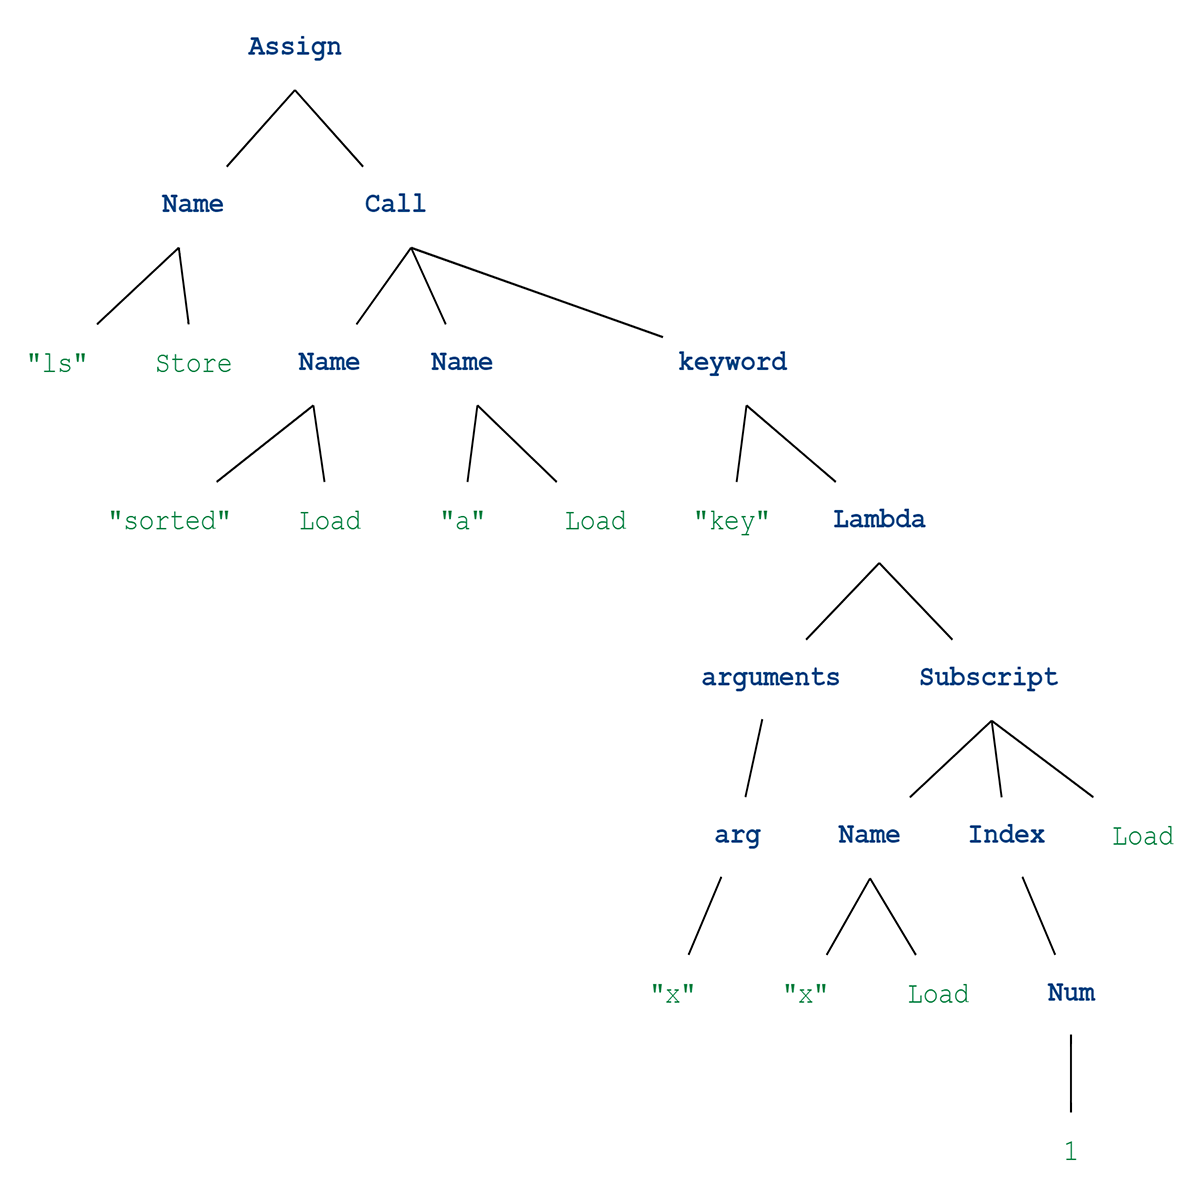
\includegraphics[width=5in]{Figures/ast}
\decoRule
\caption[Abstract Syntax Tree]{Abstract syntax tree of code snippet \code{ls = sorted(a, key=lambda x: x[1])}\protect\footnotemark.}
\label{fig:ast}
\end{figure}

\footnotetext{Picture is created with Python library \href{https://github.com/hchasestevens/show_ast}{showast}.}

The Python \emph{abstract grammar} contains a set of production rules, composed of head node and multiple child nodes. For example, in Fig \ref{fig:ast} the first rule is used to generate the assignment of statement result to variable. It consists of the head node of type \code{Assign} and two child nodes of types \code{Name} and \code{Call}, respectively. Non-terminal nodes (the blue ones) defines the general structure of the target code, while terminal nodes (the green ones) refer to symbol tokens, like variables, constants or operations. Full Python 3.6 abstract grammar can be found in Appendix \ref{AppendixA}. 

\section{Semantic parsing}
Theory of sentence analysis is derived from the idea that the words of a sentence seem to combine into patterns and structures. Each word is classified as a different in terms of its function in a sentence. According to this function, to each word there can be assigned its lexical category or part of speech, like a noun (\code{N}), adjective (\code{A}), or verb (\code{V}). 

This system could be extended to the level of syntactic categories, combining words or other syntactic categories with similar function into phrases. Each phrase is characterized by the properties of the headword that it includes. For example, the headword of the subject of a sentence is a noun, so it is classified as a noun phrase (\code{NP}). A verb is regarded as the head of the sentence predicate, so predicate is classified as a verb phrase (\code{VP}). Rules which describe how lexical categories can be combined into syntactic categories is called \emph{rewriting rules}. For example, a noun phrase category may be described as the parent of adjective and noun categories, and it may be represented by a rule of the following form:

\begin{verbatim}
NP => A N
\end{verbatim}

A formalization of such rule-based sentence structure system is called a \emph{phrase-based grammar} or \emph{constituency grammar}. Grammar is defined by the following constituents:
$V_N$ is a non terminal vocabulary, which contains the lexical and syntactic category labels;
$V_T$ is terminal vocabulary and it contains a set of words.
$P$ identifies the collection of the production rules of the grammar.
To illustrate this concept, I present a short grammar to parse a sentence \textquote{good dogs like cats} to its syntactic representation. The grammar for this example contains following vocabulary:
\begin{equation}
\begin{split}
V_N = {S, NP, VP, A, N, V}\\
V_T = {cats, dogs, like, good}
\end{split}
\end{equation}
The production rules for this grammar would be following:
\begin{verbatim}
S => NP VP
NP => A N
NP => N
VP => V NP
N => dogs
N => cats
V => like
A => good
\end{verbatim}
Graphic representation of syntactic tree  of this sentence can be seen in Fig \ref{fig:syntax_tree}.

Phrase-based grammar might also be refered as \emph{context-free grammar}, beause it provides a simple and mathematically precise mechanism for describing the methods by which phrases in some natural language are built from smaller blocks. Important features of natural language syntax such as agreement and reference are not part of the context-free grammar, but the basic recursive structure of sentences, the way in which clauses nest inside other clauses, and the way in which lists of adjectives and adverbs are swallowed by nouns and verbs, is described exactly.

\begin{figure}
\centering
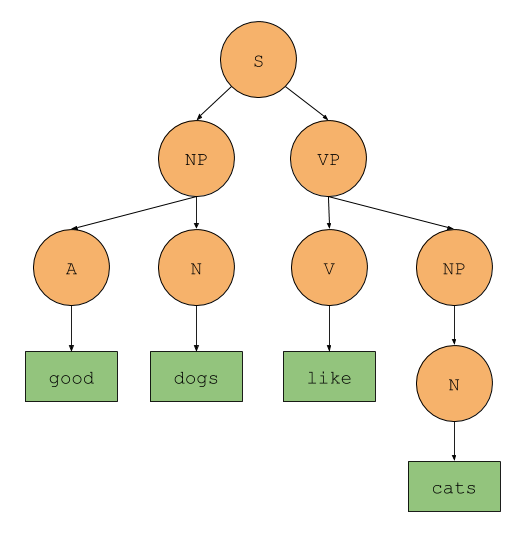
\includegraphics{Figures/syntaxtree}
\decoRule
\caption[Syntax tree]{Example of syntax tree.}
\label{fig:syntax_tree}
\end{figure}

\section{Combinatory-categorial grammar}
Phrase-structure grammars analyze the sentence recursively applying rewriting rules, starting from identification of the parts of speech or lexical categories of individual words. This rule governs how words can be combined into phrases and sentences. Compared with phrase-structure grammars, \emph{combinatory-categorial grammars} do not contain a separate collection of category-combining rules. Lexical categories of words such as adjectives and nouns describe the functions that determine how these words can combine with other categories. Each node in CCG tree can be translated into lambda calculus, thus CCG is a transparent interface between syntax and semantics of a sentence. 

Consider an example. Adjective \textquote{good} is in a category corresponding to a function that maps from the nouns into the noun phrases. The association of this item with a function looks like that:

\begin{verbatim}
good = NP/N 
\end{verbatim}

$\lambda x.good(x)$\footnote{To make connection of CCG categories with lambda calculus clear, we will complement each example of categorial operations with corresponding lines of lambda calculus.}

\code{NP} on the left side of the slash character denotes function return value and \code{N} on the right side denotes function argument. This function could be resolved with forward function application operation, denoted by character \code{>}:

\begin{verbatim}
dogs => N
good dogs => NP/N>N = NP
\end{verbatim}

$\lambda x.good(x)(DOGS)=good(DOGS)$

With backward slash character \code{\textbackslash} category on the right side denotes function return and category on the left side denotes function argument. Example:

\begin{verbatim}
bird => N
flies => N\textbackslash S
bird flies => N>N\textbackslash S = S
\end{verbatim}

$\lambda x.flies(x)$

$\lambda x.flies(x)(BIRD)=flies(BIRD) $

A verb such as \textquote{like} is usually taking two arguments and associated as follows:

\begin{verbatim}
like => (S/NP) \\ N
cats => N
like cats => (S/NP) \\ N>N = S/NP
\end{verbatim}

$\lambda x.\lambda y.like(x, y)$

$\lambda x.\lambda y.like(y, x)(CATS)=\lambda y.like(y, CATS)$

The function \code{(S/NP)\\N} maps \code{N} to a range of functions of form \code{S/NP}.  Character \code{<} denotes backward function application. Final sentence example:

\begin{verbatim}
good dogs => NP
like cats => S/NP
good dogs like cats => NP<S/NP = S
\end{verbatim}

$\lambda y.like(y, CATS)$

$\lambda y.like(y, CATS)(good(DOGS))=like(good(DOGS), CATS)$

\section{Dependency parsing}

\begin{figure}[h]
\centering
\includegraphics[width=5in]{Figures/dependency_graph}
\decoRule
\caption[Syntax tree]{Dependency graph for sentence \textquote{nice dogs like cats}\protect\footnotemark.}
\label{fig:dependency_graph}
\end{figure}

\footnotetext{Picture is created in \href{http://grammarscope.sourceforge.net/}{GrammarScope}.}

Another approach to represent sentence semantical structure is \emph{dependency parsing}. \emph{Dependency grammar} is different from constituency grammars like CFG or CCG, which build sentence tree by applying rewrite rules to constitute high level phrases from low level syntactic categories and lexems. It also defines sentence structure as a graph, but without phrasal nodes like \code{NP} or \code{VP}. Instead each node represent one word which points to it dependent. Since such representation do not rely on established phrase word order it is well suited for the analysis of languages with free word order, such as Ukrainian.



In Fig \ref{fig:dependency_graph} sentence \textquote{nice dogs like cats} parsed to dependency graph. It consists of following dependencies: 

\begin{verbatim}
amod = adjectival modifier
nmod = nominal modifier
case = case marker
\end{verbatim}

\section{Word embeddings}

\begin{figure}[h]
\centering
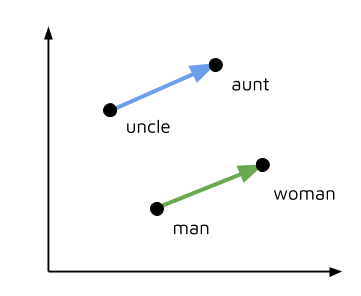
\includegraphics{Figures/word_embeddings}
\decoRule
\caption[Word vectors]{Example of collinearity between two word vectors.}
\label{fig:word_embeddings}
\end{figure}

The task of language modeling requires the transformation of words and documents into vector representation. Simple tasks like text classification could be done using naive representations like a bag of words or one hot encoding. However, these approaches would require excessive memory usage to handle large vocabulary and usually do not infer existing semantical connections between words in a language. 



Methods of \emph{word embeddings} solve both problems, providing dense vectors of real numbers, which represent word positions in $n$-dimensional space. This space represents contextual similarity of the words, thus word embeddings support semantic relations as vector operations. For example, adding vector ‘woman’ to vector ‘uncle’ and subtracting vector ‘man’ will result in vector approximately pointing to the same point as vector ‘aunt’ (see Fig \ref{fig:word_embeddings} for example).

\section{Long-short term memory network}
Model of LSTM network is an extension of the simple recurrent network. It can store values in the hidden layer for a short or long period of time because it uses no activation function within its recurrent components. This makes it possible to backpropagate error gradient through long sequences of data without gradient vanishing or gradient exploding.

At the time step $t$ LSTM consumes previous value of hidden state $h^{(t-1)}$, memory cell $c^{(t-1)}$ and input vector $x^{(t)}$. The new value of memory cell uses gates to forget part of previous value and remember new value. Forget gate calculation:

\begin{equation}
f^{(t)} = \sigma(W_f\cdot[h^{(t-1)},x^{(t)}] + b_f)
\label{lstm:ft}
\end{equation} 

Input gate:
\begin{equation}
i^{(t)}=\sigma(W_i\cdot[h^{(t-1)}, x^{(t)}]+b_i)
\label{lstm:input}
\end{equation} 

\begin{figure}[h]
\centering
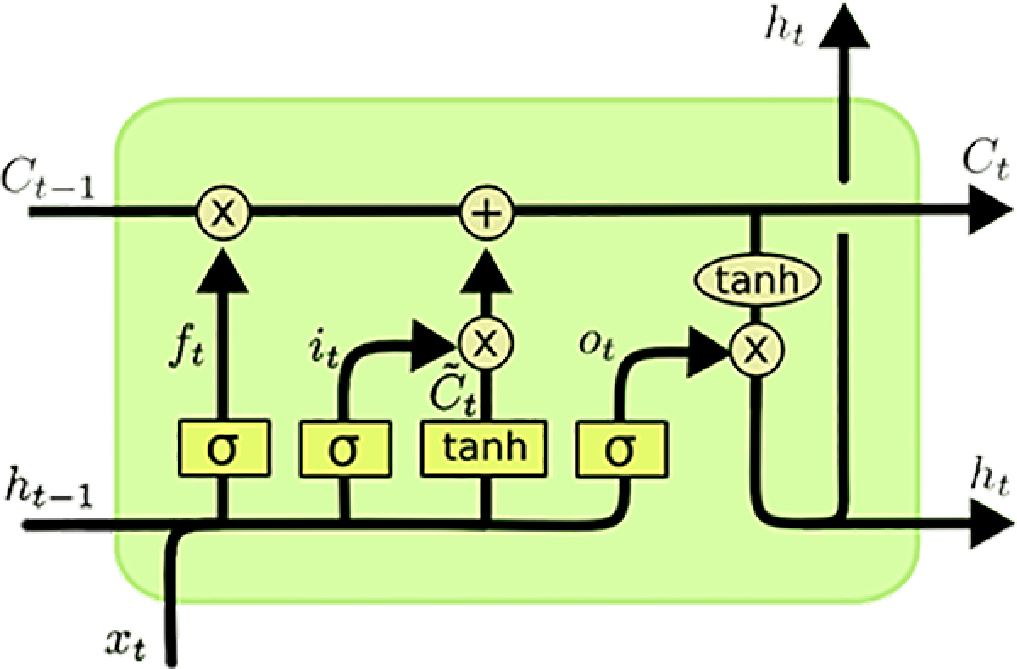
\includegraphics{Figures/lstm}
\decoRule
\caption[Long-short term memory]{Long-short term memory network achitecture \parencite{lstm-picture}.}
\label{fig:word_embeddings}
\end{figure}

New memory state ($\circ$ denotes entrywise product):
\begin{equation}
\begin{gathered}
\widetilde{C}^{(t)} = tanh(W_c\cdot[h^{(t-1)}, x^{(t)}]+b_C) \\

C^{(t)} = f_t\circ C^{(t-1)}+i_t\circ\widetilde{C}^{(t)}
\end{gathered}
\label{lstm:c}
\end{equation} 

New hidden state:
\begin{equation}
\begin{gathered}
o^{(t)}=\sigma(W_o[h^{(t-1)},x^{(t)}]+b_o) \\

h^{(t)}=o^{(t)}\circ tanh(C^{(t)})
\end{gathered}
\label{lstm:h}
\end{equation} 

\section{Sequence-to-sequence machine translation with attention}
% http://phontron.com/class/mtandseq2seq2017/mt-spring2017.chapter8.pdf
The task of machine translation can be formalized as mapping of a sequence of words in a source language to a sequence of words in a target language. This task can be solved with an \emph{encoder-decoder} model, which consists of two RNNs. The first RNN consumes input sequence step by step and encodes it into so-called thought vector. After encoding, the second RNN uses thought vector as its initial hidden state and decodes output sentence word by word.  Each word from decoder output is used as input for the next decoding step until the model outputs the end-of-sentence token. 

Theoretically, a sufficiently large encoder-decoder model should be able to perform machine translation perfectly. However, to encode all words and dependencies between them in the arbitrary-length sentences the thought vector should have enormous length. It would require massive computational resources to train and use such architecture, and thus this approach is ineffective.

This problem can be solved with attention technique. Its basic idea is to replace single vector representation of input sentence with references to representations of different words in it. On the encoding step, each word representation $h_e(t)$ is stored as a column of matrix $H_e$. During the decoding step, hidden state of decoder network is calculated as follows:

\begin{equation}
h_d(t) = enc([embed(w(t));c(t-1)], h_d(t-1))
\label{attn:hd}
\end{equation}

\begin{figure}
\centering
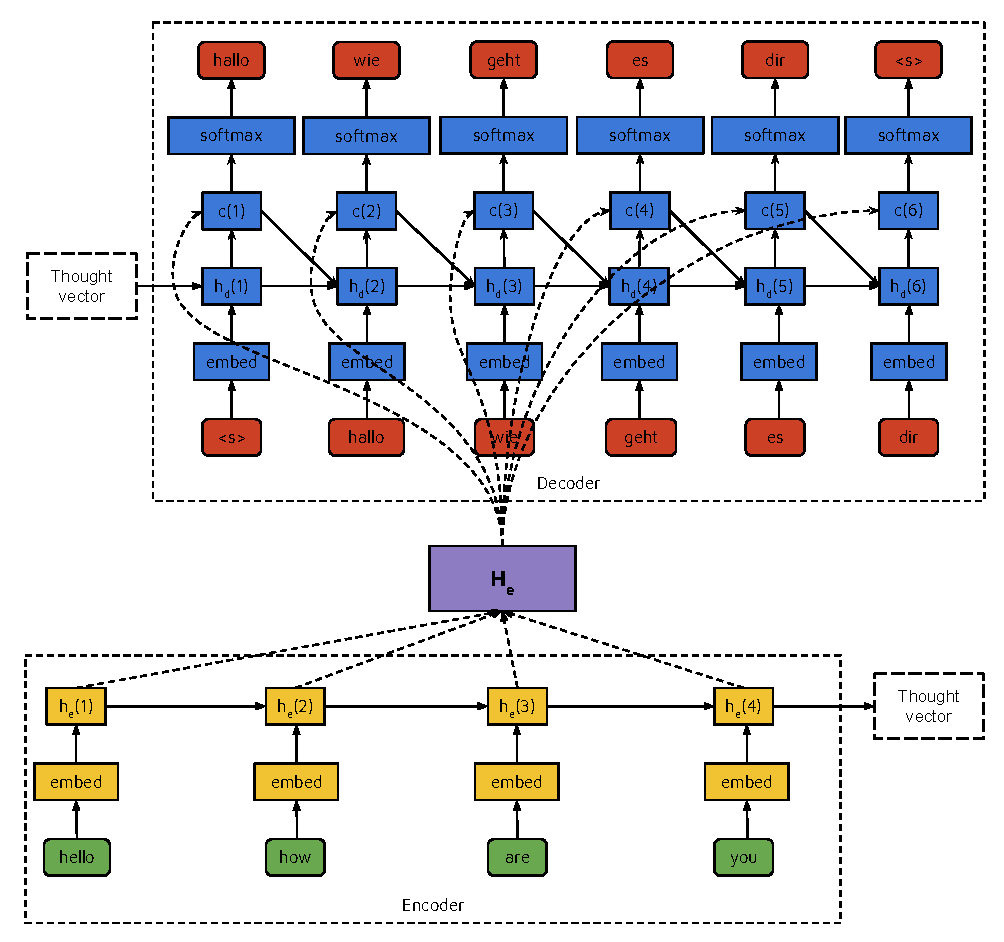
\includegraphics[width=5in]{Figures/seq2seq.pdf}
\decoRule
\caption[Seq2Seq model]{Seq2Seq with attention model.}
\label{fig:seq2seq}
\end{figure}

Elements of attention vector are calculated with arbitrary attention score function (for example, vector product) for each pair of decoder and encoder representations:
\begin{equation}
\alpha_j(t) = attnscore(h_e(j), h_d(t))
\label{attn:alpha}
\end{equation}

\begin{equation}
\alpha_j(t) = softmax(\alpha_j(t))
\label{attn:alpha2}
\end{equation}

Then context vector is calculated as a weighted sum of encoder representations:
\begin{equation}
	c(t) = H_e\cdot\alpha(t)
	\label{attn:c}
\end{equation}

\begin{equation}
	P(t) = softmax(W_{hs}\cdot[h_d(t);c(t)])
\label{attn:P}
\end{equation}

This way each decoder step can use information from arbitrary part of encoded sequence. Input sentence representation should not be limited to fixed length thought vector, and thus it can model natural language with adequate model size. An architecture of sequence-to-sequence model with attention can be seen in Fig \ref{fig:seq2seq}.

\section{Recursive neural networks}

% reflects domain knowledge
The architecture of recurrent neural network contains inductive bias about conditional probability of target variable with previous values in a sequence. Representation of natural language can also be modeled as a plain sequence of words. However, this approach ignores domain knowledge about the syntactic structure of a text. A syntactic tree contains important information about relations between individual terms and thus should not be omitted in the task of natural language meaning representation.

\begin{figure}[h]
\centering
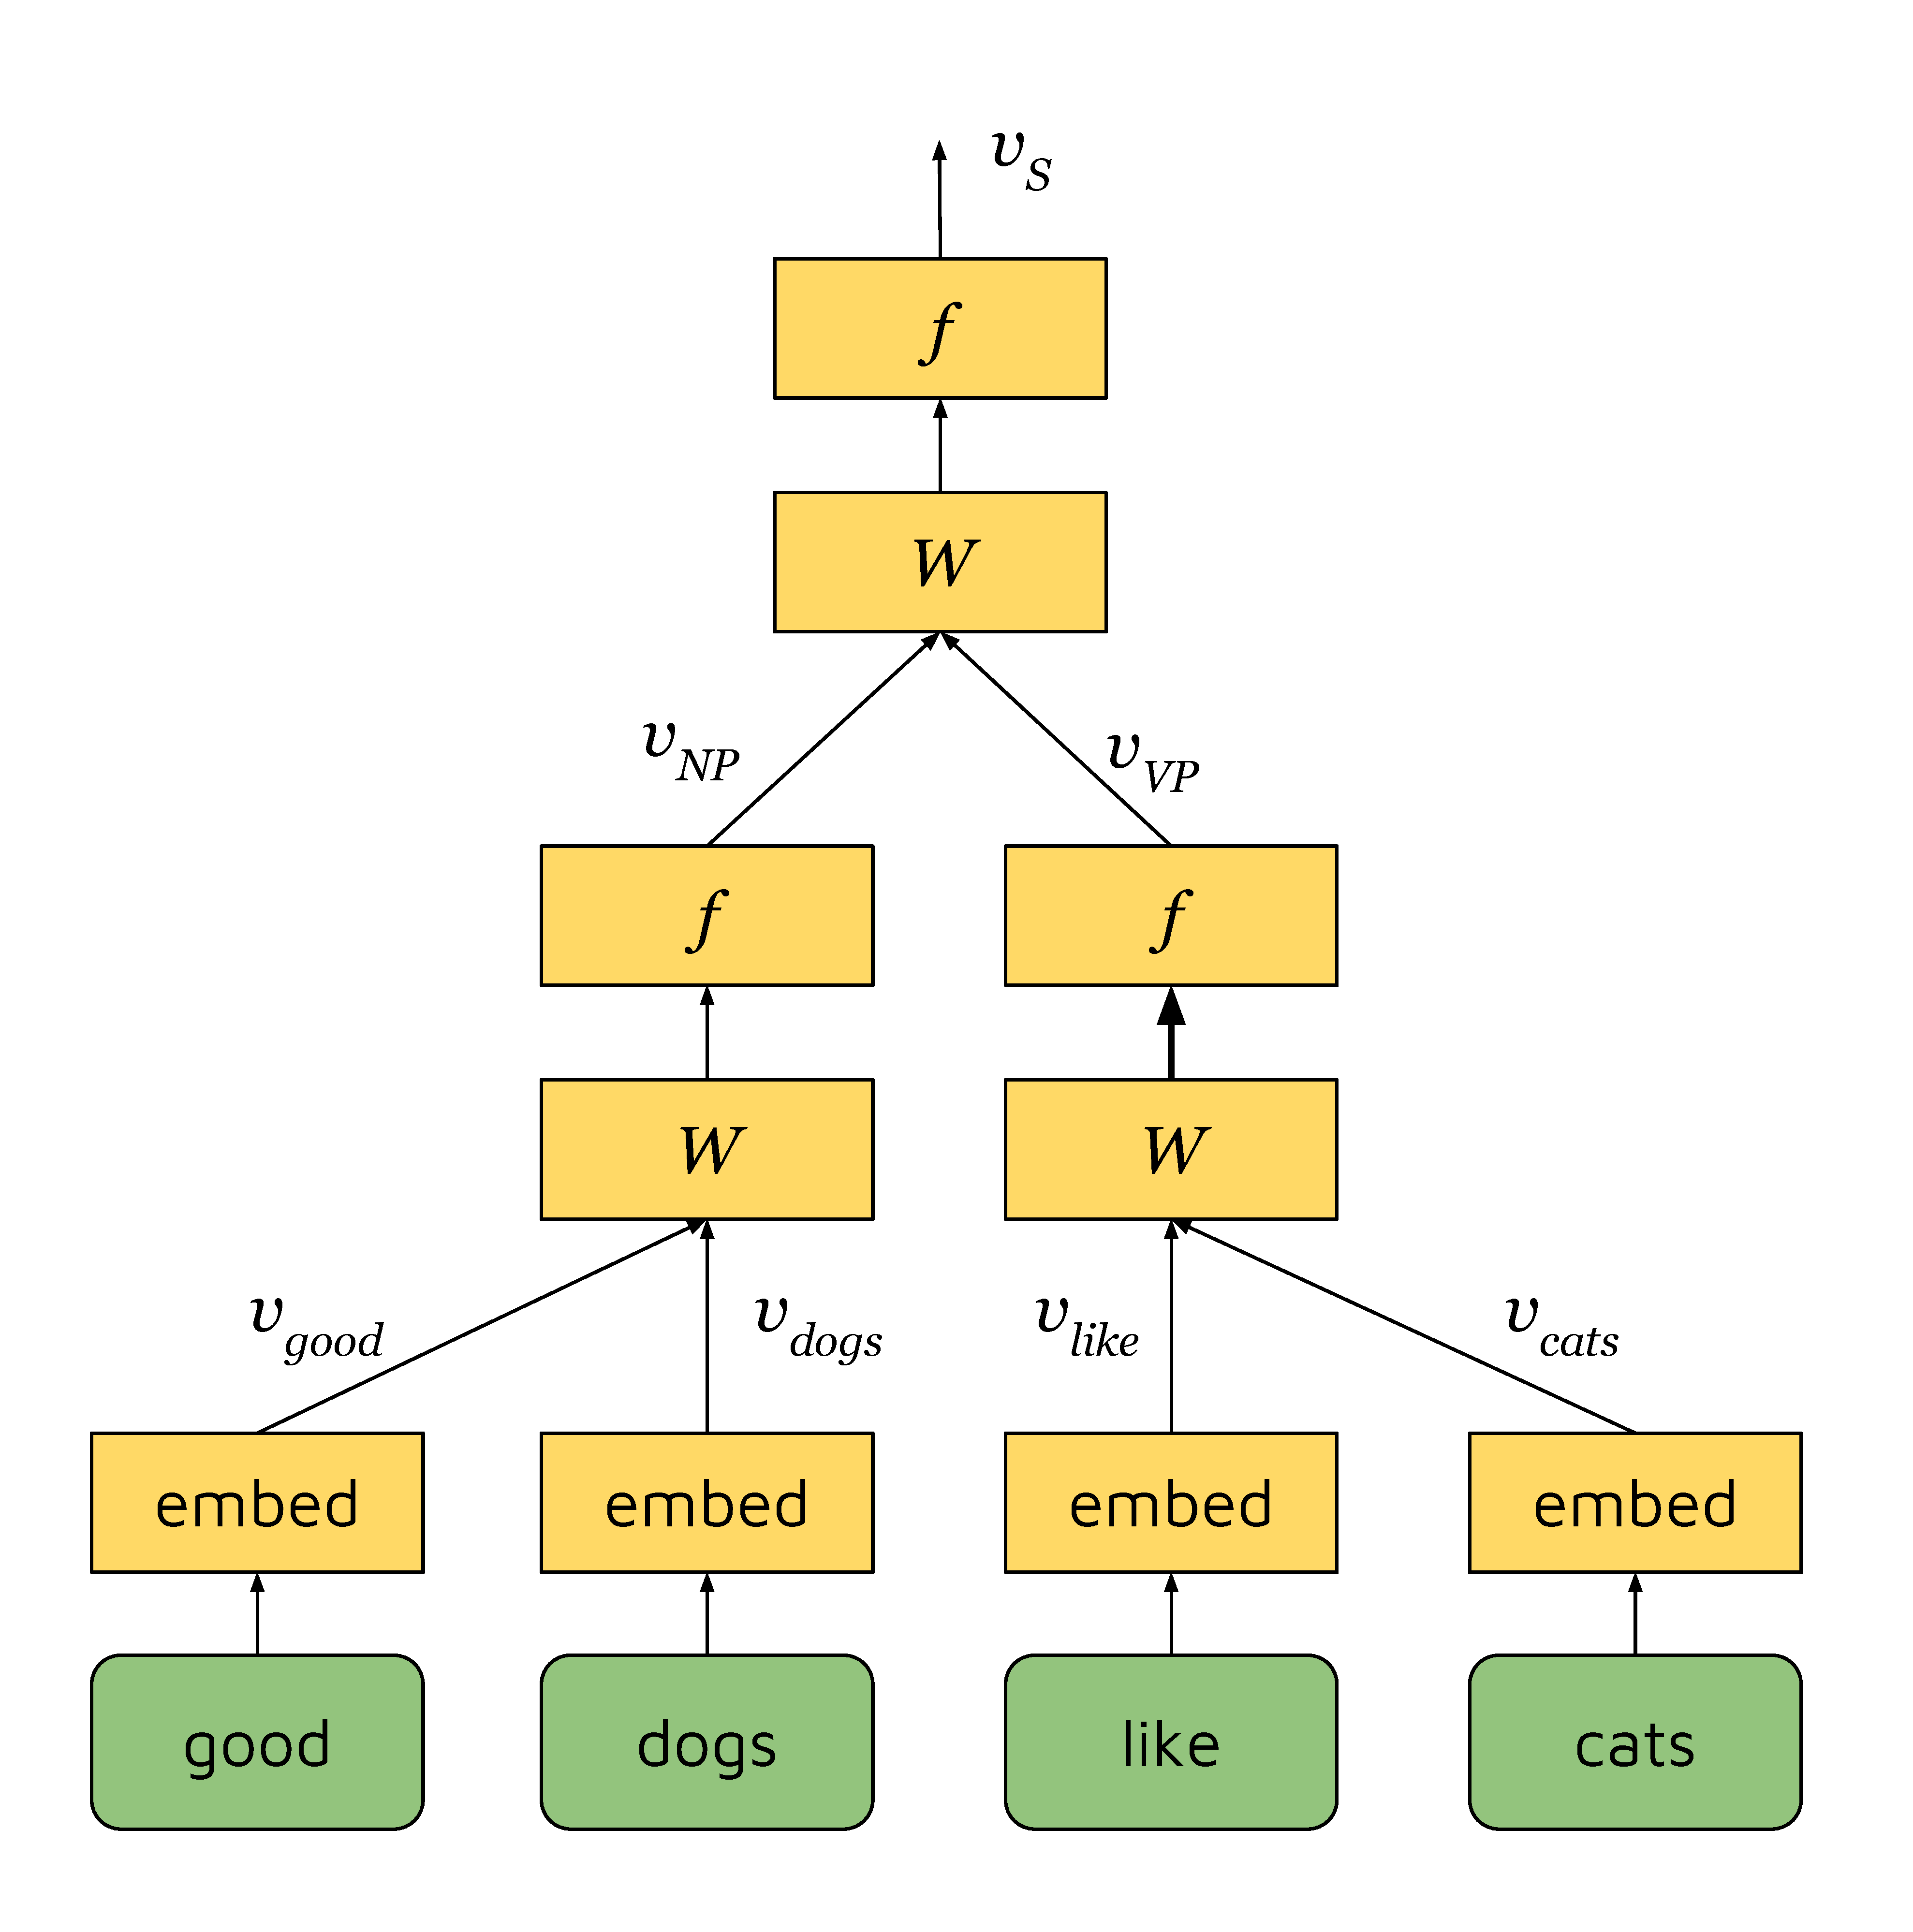
\includegraphics{Figures/rvnn}
\decoRule
\caption[RvNN flow]{Examle of recursive neural network flow.}
\label{fig:rvnn}
\end{figure}

Topological structures with variable length could be modeled by neural networks recursively applying the same set of weights to each node. To model syntactic tree, each word is represented by corresponding embedding vector and then parent vectors are computed using a bottom-up approach with composition functions. For example, representation of the syntactic tree of sentence \textquote{good dog like cats} could be modeled i the following way:
\begin{equation}
\begin{split}
v_{NP} = f(W\cdot[v_{good}, v_{dog}])\\
v_{VP} = f(W\cdot[v_{like}, v_{cats}])\\
v_S = f(W\cdot[v_{NP}, v_{VP}])
\label{rvnn:example}
\end{split}
\end{equation}
where $f$ is any differentiable non-linearity like $tanh$ or $ReLU$. The example of semantic tree parsing with recursive network is presented in Fig \ref{fig:rvnn}.

\section{Pointer networks}
Neural network operates with vector representations of words which selected from predefined vocabulary. This imposes the problem of unknown words which don't have vector representation. This is especially important for the translation task where both input and output sequences could contain rare, special words or names. However, names of people or locations should not be translated but copied to target sequence. \cite{Vinyals2015} proposed solution of this problem with \emph{pointer network}. For each decoding step it calculates the probability of next word to be copied from an input sequence. Calculation of this probability described below step-by-step.

Let's denote $H_{encoder}$ as a matrix of encoder output vectors and $h_{decoder}^{(t)}$ - decoder output vector on decoding step $t$. First is calculated hidden state of pointer network:

\begin{equation}
    \begin{gathered}
    
    H_{enc.pointer} = H_{encoder} \cdot W_{encoder}\\
    
    h_{dec.pointer} = h_{decoder}^{(t)} \cdot W_{decoder}\\
    
    H_{pointer} = tanh(H_{enc.pointer} + h_{dec.pointer})\\
    
    \end{gathered}
    \label{eq:pointer}
\end{equation}

Then each row from matrix $H_{pointer}$ is translated to one value and probability calculated as result of $softmax$:

\begin{equation}
    \begin{gathered}
    
    H_{prob} = H_{pointer} \cdot W_{pointer}\\
    
    P = softmax(H_{prob})\\
    
    \end{gathered}
\end{equation}


